\documentclass{lug}

\title{GPU Computing}
\author{Sam Sartor}
\institute{Mines Linux Users Group}

\usepackage{etoolbox}
\usepackage{array}
\usepackage{amsmath}
\usepackage{adjustbox}
\usepackage{calc}
\usepackage{lmodern}

\makeatletter
\patchcmd{\beamer@sectionintoc}{\vskip1.5em}{\vskip0.5em}{}{}
\makeatother

\newcommand{\pmidg}[1]{\parbox{\widthof{#1}}{#1}}
\newcommand{\splitslide}[4]{
    \noindent
    \begin{minipage}{#1 \textwidth - #2 }
        #3
    \end{minipage}%
    \hspace{ \dimexpr #2 * 2 \relax }%
    \begin{minipage}{\textwidth - #1 \textwidth - #2 }
        #4
    \end{minipage}
}

\begin{document}

\section{The GPU}

\begin{frame}{What is a GPU?}
    \splitslide{0.65}{.7em}{

        A Graphics Processing Unit (GPU) is a specialized chip primarily for
        accelerating graphical calculations.

        \vspace{2ex}

        GPUs generally derive their performance from their ability to do large
        numbers of identical arithmetic calculations in parallel.

    }{
        \pmidg{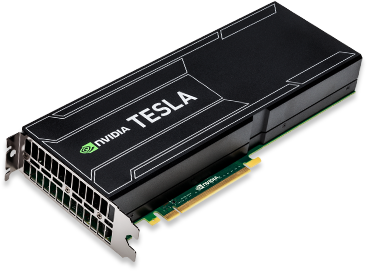
\includegraphics[width=\textwidth]{graphics/tesla}}
    }
\end{frame}

\begin{frame}{GPUs for Graphics}
    \splitslide{0.75}{.7em}{

        Screens have lot of pixels that need to be calculated very quickly.
        All of the required calculations are identical, just with different
        input numbers. And because pixels are independent the calculations are
        also trivial to parallelize. As a result, using the unnecessarily
        clever CPU would be wasteful and slow. A separate  pixel-optimized
        chip can be used instead, leaving the CPU to do the important stuff.

    }{
        \pmidg{
\includegraphics[width=\textwidth]{graphics/pixels}}
    }
\end{frame}

\begin{frame}{GPU Computing}
    \splitslide{0.75}{.7em}{

        Coloring pixels is not the only problem that involves a large number
        of similar, repetitive calculations. General-purpose GPUs can be used
        for countless other problems including machine learning, computer
        vision, signal processing, statistics, linear algebra, finance, and
        cryptography.

    }{
        \pmidg{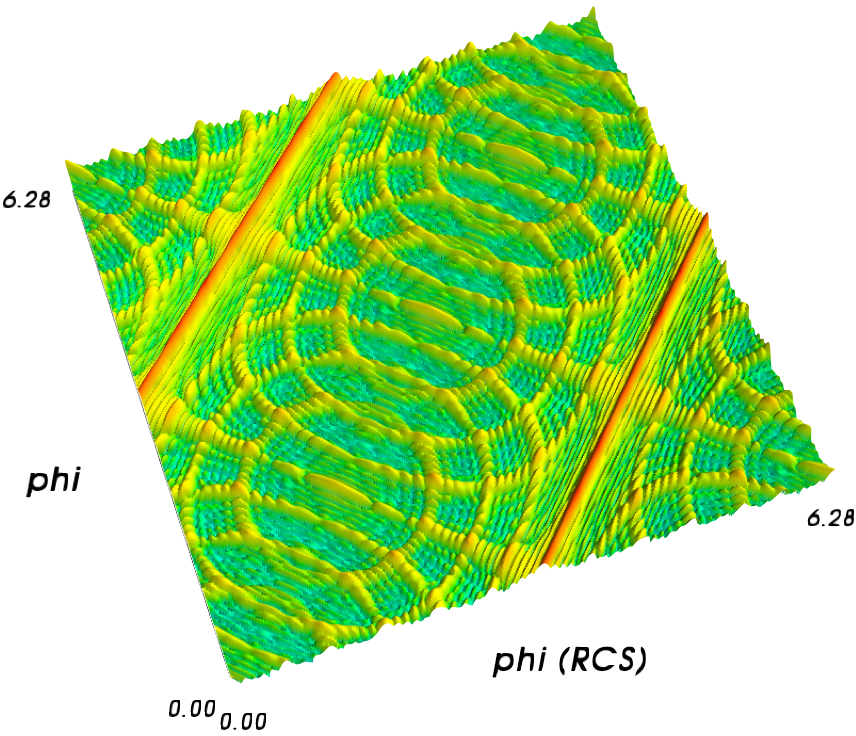
\includegraphics[width=\textwidth]{graphics/resimg}}
    }
\end{frame}

\begin{frame}{History}
    \splitslide{0.75}{.7em}{

        \emph{1970s} - Highly specialized, used only for buffering video and drawing
        simple 2D rasters (sprites)

        \emph{1980s} - Common bitmap operations such as filling simple 2D shapes

        \emph{1990s} - 3D triangular graphics, common interfaces (OpenGL, Direct3D)
        developed

        \emph{2000s} - General purpose GPUs, capable of executing arbitrary
        instructions

        \emph{2010s} - Highly general, used as much for supercomputing as for
        graphics

    }{
        \pmidg{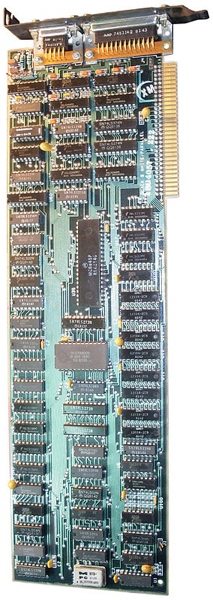
\includegraphics[width=\textwidth]{graphics/ibm-pc-mda}}
    }
\end{frame}

\section{GPU Operation}

\section{Machine Learning}

\section{Computing At Home}

\begin{frame}{OpenGL Shaders}
    \splitslide{0.75}{.7em}{

        Although shaders are used for pixel stuff, they are still
        fundamentally general purpose. Use vertex attributes, uniforms, and
        textures as input. Use the framebuffer for output.

    }{
        \pmidg{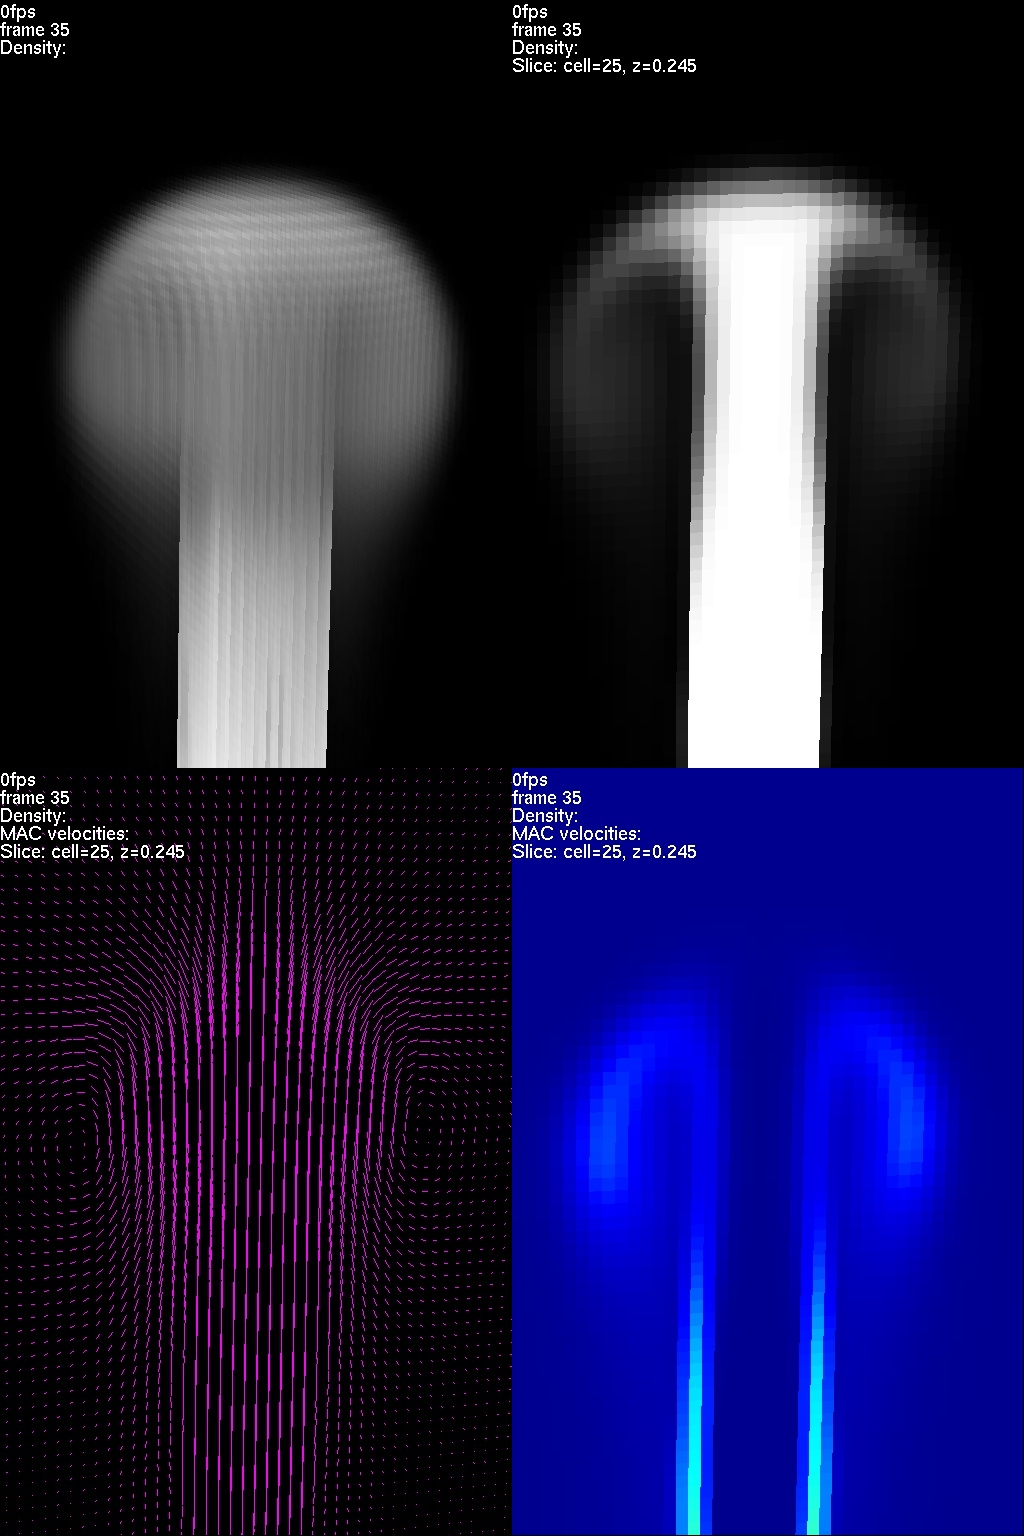
\includegraphics[width=\textwidth]{graphics/shaderfluid}}
    }
\end{frame}

\begin{frame}{OpenGL Shaders - Pros \& Cons}
    \textbf{Pros}

    \begin{itemize}
        \item Shaders have been around since like 2004
        \item Universally supported
        \item OpenGL allows for minimal setup
    \end{itemize}

    \textbf{Cons}

    \begin{itemize}
        \item Low level
        \item Not very general
        \item All data has to be stored in textures/images
    \end{itemize}
\end{frame}

\begin{frame}{CUDA}
    \splitslide{0.75}{.7em}{

        CUDA is a computing platform and API that provides truly general GPU
        computing. C/C++/Fortran code can be compiled ahead of time or at
        runtime and sent to the GPU along with arbitrary chunks of memory.

        \vspace{2ex}

        Libraries for controlling and communicating with CUDA programs exist
        for many languages including C/C++ (through the CUDA SDK) and Python
        (PyCUDA library).

    }{
        \pmidg{
\includegraphics[width=\textwidth]{graphics/nvidia-cuda}}
    }
\end{frame}

\begin{frame}{CUDA - Pros \& Cons}
    \textbf{Pros}

    \begin{itemize}
        \item Get to use real C/C++
        \item Pointers, recursion, etc.
        \item Copy arbitrary data between CPU and GPU
        \item Fast
    \end{itemize}

    \textbf{Cons}

    \begin{itemize}
        \item Only available on high-end Nvidia cards
        \item Very low level
        \item Annoying to setup
    \end{itemize}
\end{frame}

\begin{frame}{OpenCL}
    \splitslide{0.75}{.7em}{

        OpenCL is a cross platform alternative to CUDA. It is similar in
        structure to OpenGL, but intended for general-purpose computation (not
        just 3D graphics). Bindings exist for all common languages.

    }{
        \pmidg{
\includegraphics[width=\textwidth]{graphics/opencl-logo}}
    }
\end{frame}

\begin{frame}{OpenCL - Pros \& Cons}
    \textbf{Pros}

    \begin{itemize}
        \item Cross platform
        \item Nice API
        \item Will use CPU instead of GPU if needed (works anywhere)
    \end{itemize}

    \textbf{Cons}

    \begin{itemize}
        \item Must use C-like OpenCL language
        \item No recursion, pointers, etc.
        \item Slightly slower than CUDA
    \end{itemize}
\end{frame}

\section{ArrayFire}

\section{Torch}

\section{TensorFlow}

\end{document}